%% Chapter-1.tex
%% Mac Radigan
%
%% Examples from SICP Chapter 1

    \section{Building Abstractions with Procedures}
        \subsection{The Elements of Programming}
            \subsubsection{Expressions}
Exercise 1.1. Below is a sequence of expressions. What is the result printed by the interpreter in response to each expression? Assume that the sequence is to be evaluated in the order in which it is presented.
\newline
              \schemelist{../chapter-1/sicp_ch1_e1-1.scm}
              \outlist{../output/sicp_ch1_e1-1.out}
            \subsubsection{Naming and the Environment}
Exercise 1.2. Translate the following expression into prefix form
\newline
\begin{equation}
\frac{5 + 1/2 + \left(2 - \left(3 - \left(6 + 1/5\right) \right) \right)}{3 \left( 6 - 2 \right) \left( 2 - 7 \right)}
\end{equation}
\newline
              \schemelist{../chapter-1/sicp_ch1_e1-2.scm}
              \outlist{../output/sicp_ch1_e1-2.out}
            \subsubsection{Evaluating Combinations}
Exercise 1.3. Define a procedure that takes three numbers as arguments and returns the sum of the squares of the two larger numbers.
\newline
              \schemelist{../chapter-1/sicp_ch1_e1-3.scm}
              \outlist{../output/sicp_ch1_e1-3.out}
            \subsubsection{Compound Procedures}
Exercise 1.4. Observe that our model of evaluation allows for combinations whose operators are compound expressions. Use this observation to describe the behavior of the following procedure:
\newline
\text{(define (a-plus-abs-b a b)}
\newline
\text{((if ($<$ b 0) + -) a b))}
\newline
              \schemelist{../chapter-1/sicp_ch1_e1-4.scm}
              \outlist{../output/sicp_ch1_e1-4.out}
            \subsubsection{The Substitution Model for Procedure Application}
Exercise 1.5. Ben Bitdiddle has invented a test to determine whether the interpreter he is faced with is using applicative-order evaluation or normal-order evaluation. He defines the following two procedures:
\newline
\text{(define (p) (p))}
\newline
\text{  (define (test x y)}
\newline
\text{    (if (= x 0)}
\newline
\text{    0}
\newline
\text{    y))}
\newline
Then he evaluates the expression
\newline
\text{(test 0 (p))}
\newline
What behavior will Ben observe with an interpreter that uses applicative-order evaluation? What behavior will he observe with an interpreter that uses normal-order evaluation? Explain your answer.  (Assume that the evaluation rule for the special form if is the same whether the interpreter is using normal or applicative order: The predicate expression is evaluated first, and the result determines whether to evaluate the consequent or the alternative expression.)
\newline

              % infinite loop (do not include output listing)
              \schemelist{../chapter-1/sicp_ch1_e1-5.scm}
              \outlist{../output/sicp_ch1_e1-5.out}
            \subsubsection{Conditional Expressions and Predicates}
            \subsubsection{Example: Square Roots by Newton's Method}
Exercise 1.7. The good-enough? test used in computing square roots will not be very effective for finding the square roots of very small numbers. Also, in real computers, arithmetic operations are almost always performed with limited precision. This makes our test inadequate for very large numbers. Explain these statements, with examples showing how the test fails for small and large numbers. An alternative strategy for implementing good-enough? is to watch how guess changes from one iteration to the next and to stop when the change is a very small fraction of the guess. Design a square-root procedure that uses this kind of end test. Does this work better for small and large numbers?
\newline

Newton's method:
\begin{equation}
x_{n+1} = x_{n} - \frac{f\left(x_n\right)}{f^{'}\left(x_n\right)}
\label{eq:newtons}
\end{equation}

Applied to square root:
\begin{equation}
x_{n+1} 
= x_{n} - \frac{x^2_n - \mbox{guess}}{2 x_n}
\label{eq:newtons_sqrt}
\end{equation}

              \schemelist{../chapter-1/sicp_ch1_e1-7.scm}
              \outlist{../output/sicp_ch1_e1-7.out}
            \subsubsection{Procedures as Black-Box Abstractions}
        \subsection{Procedures and the Processes They Generate}
            \subsubsection{Linear Recursion and Iteration}
Exercise 1.9: Each of the following two procedures defines a method for adding two positive integers in terms of the procedures inc, which increments its argument by 1, and dec, which decrements its argument by 1.
\newline
              \schemelist{../chapter-1/sicp_ch1_e1-9.scm}
              \outlist{../output/sicp_ch1_e1-9.out}

Exercise 1.11: A function f is defined by the rule that 

\begin{equation}
f\left(n\right) = 
\begin{cases}
n & n < 3 \\
1 f\left(n-1\right) + 2 f\left(n-2\right) + 3 f\left(n-3\right) & \mbox{ otherwise }
\end{cases}
\label{eq:ss_recursive}
\end{equation}

Write a procedure that computes f by means of a recursive process. Write a procedure that computes f by means of an iterative process.
\newline

Representing State Space Transitions
\newline

Direct Iterative Implementation
\newline

\begin{equation}
f\left(n\right) \coloneqq s_0
\label{eq:direct_def}
\end{equation}

with state transition

\begin{equation}
\stackrel{\mbox{T}}{
\left[ \begin{array}{c}
s_0 \leftarrow s_0 + 2 s_1 + 3 s_2 \\
s_1 \leftarrow s_0 \\
s_2 \leftarrow s_1 \\
\end{array} \right]
}
\label{eq:direct_trans}
\end{equation}

and initial conditions

\begin{equation}
\stackrel{\mbox{$S_0$}}{
\left[ \begin{array}{c}
s_0 \coloneqq 2 \\
s_1 \coloneqq 1 \\
s_2 \coloneqq 0 \\
\end{array} \right]
}
\label{eq:direct_init}
\end{equation}

Linear Feedback Shift Register (LFSR) representation
\newline

\begin{equation}
f\left(n,\underbar{s}\right)
\leftarrow
\begin{cases}
n^{th}_1 \underbar{s} & n = 0 \\
f\left( n-1, n^{th}_1 \leftangle \sigma_{1}(\underbar{s}), \left[ 1,2,3 \right] \rightangle \right) & \mbox{ otherwise }
\end{cases}
\label{eq:lfsr_def}
\end{equation}

\begin{equation}
\leftangle x, y \rightangle
\triangleq
\sum_{k} x_k y_k 
= x_k y^k
\label{eq:dotprod}
\end{equation}

\begin{equation}
n^{th}_k
\triangleq
x_k
\label{eq:nth}
\end{equation}

\begin{equation}
\sigma_k \left( \underbar{x} \right)
\triangleq
x_{\left( n + k \right) mod |x|} \forall n \in \underbar{x}
\label{eq:rotate}
\end{equation}

\begin{figure}[H]
\begin{center}
%\resizebox{7in}{!}{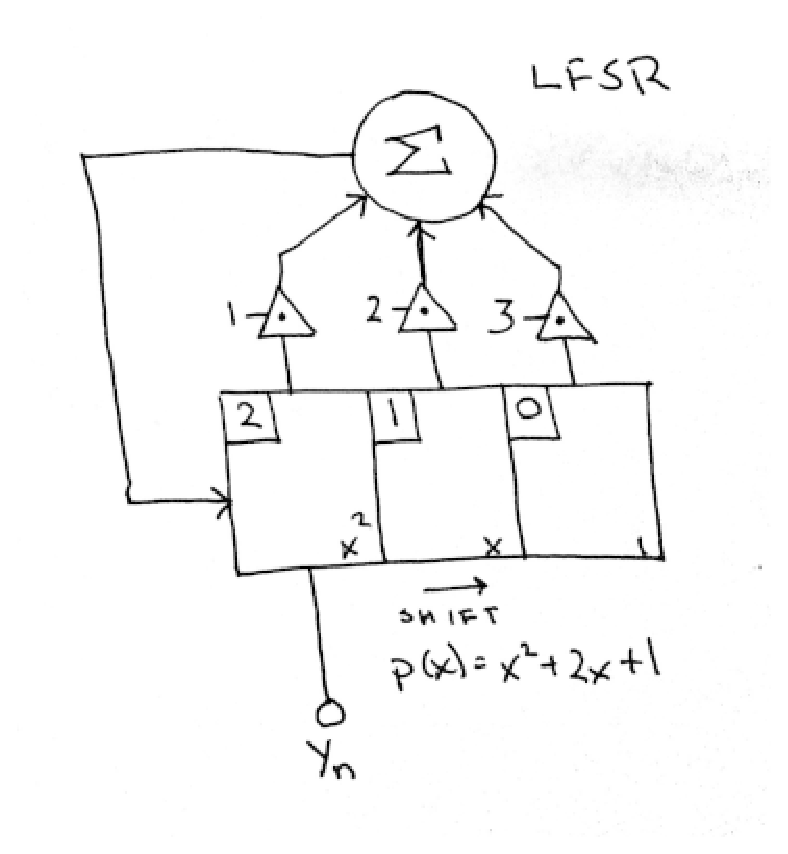
\includegraphics{./figures/lfsr-2.eps}
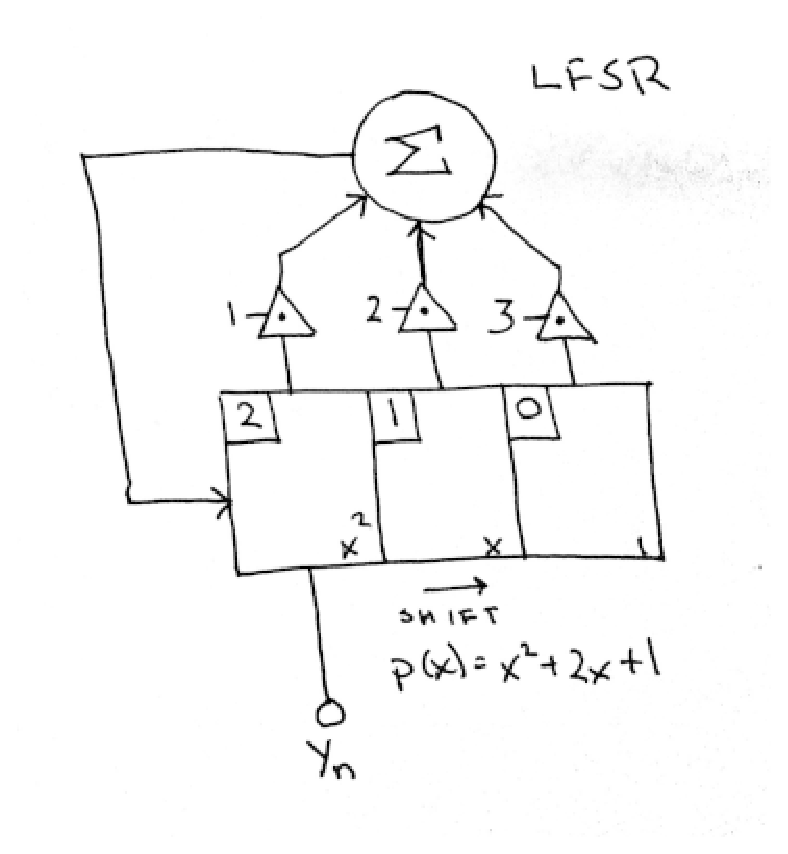
\includegraphics{./figures/lfsr-2.eps}
\end{center}
\caption{Linear Feedback Shift Register (LFSR)}
\label{fig:lfsr}
\end{figure}

State Space Representation
\newline

\begin{equation}
\mathbf{X}_k = \mathbf{F}\mathbf{X}_{k-1}
\label{eq:ss_rep}
\end{equation}

\begin{equation}
\stackrel{\mbox{$X_k$}}{
\left[ \begin{array}{c}
x^{'}_{0} \\
x^{'}_{1} \\
x^{'}_{2} \\
\end{array} \right]
}
= 
\stackrel{\mbox{$F$}}{
\left[ \begin{array}{ccc}
1 & 2 & 3 \\
1 & 0 & 0 \\
0 & 1 & 0 \\
\end{array} \right]
}
\stackrel{\mbox{$X_{k-1}$}}{
\left[ \begin{array}{c}
x_{0} \\
x_{1} \\
x_{2} \\
\end{array} \right]
}
\label{eq:ss_rep_2}
\end{equation}

where

\begin{equation}
\mathbf{X}_0 = 
\stackrel{\mbox{$X_{0}$}}{
\left[ \begin{array}{c}
2 \\
1 \\
0 \\
\end{array} \right]
}
\label{eq:ss_x0}
\end{equation}

so

\begin{equation}
\mathbf{X}_k 
= \mathbf{F}\mathbf{X}_{k-1}
= \mathbf{F} \left( \mathbf{F}\mathbf{X}_{k-2} \right)
= \mathbf{F} \left( \mathbf{F} \left( \mathbf{F}\mathbf{X}_{k-3} \right) \right)
= \cdots
= \mathbf{F}^N \mathbf{X}_0
\label{eq:ss_rep_expanded}
\end{equation}

              \schemelist{../chapter-1/sicp_ch1_e1-11.scm}
              \outlist{../output/sicp_ch1_e1-11.out}
            \subsubsection{Tree Recursion}
            \subsubsection{Orders of Growth}
            \subsubsection{Exponentiation}
Exercise 1.16:  Design a procedure that evolves an iterative exponentiation process that uses successive squaring and uses a logarithmic number of steps, as does fast-expt.  (Hint: Using the observation that $\left(b^{\frac{n}{2}}\right)^2 = \left(b^2\right)^{\frac{n}{2}}$, keep, along with the exponent n and the base b, an additional state variable a, and define the state transformation in such a way that the product a bn is unchanged from state to state. At the beginning of the process a is taken to be 1, and the answer is given by the value of a at the end of the process. In general, the technique of defining an invariant quantity that remains unchanged from state to state is a powerful way to think about the design of iterative algorithms.)

\begin{equation}
f_{benchmark}\left(x,n\right) =
\begin{cases}
1 & \mbox{ if n is zero } \\
f_{benchmark}\left(x,\frac{n}{2}\right)^{2} & \mbox{ if n is even, nonzero } \\
f_{benchmark}\left(x,n-1\right)^{2} & \mbox{ if n is odd }
\end{cases}
\label{eq:fast_expt_benchmark}
\end{equation}

may be restructured as

\begin{equation}
f\left(x,n\right) = f_{k}\left(x,n,p\right)
\label{eq:fast_expt_fast}
\end{equation}

where

\begin{equation}
f_{k}\left(x,n,p\right) =
\begin{cases}
p & \mbox{ if n is zero } \\
f_{k}\left(x,\frac{n}{2},p\right) & \mbox{ if n is even, nonzero } \\
f_{k}\left(x,n-1,p \cdot x\right) & \mbox{ if n is odd }
\end{cases}
\label{eq:fast_expt_fast_recur}
\end{equation}

              \schemelist{../chapter-1/sicp_ch1_e1-16.scm}
              \outlist{../output/sicp_ch1_e1-16.out}
            \subsubsection{Greatest Common Divisors}
            \subsubsection{Example: Testing for Primality}
        \subsection{Formulating Abstractions with Higher-Order Procedures}
            \subsubsection{Procedures as Arguments}
            \subsubsection{Constructing Procedures Using Lambda}
            \subsubsection{Procedures as General Methods}
            \subsubsection{Procedures as Returned Values}
Exercise 1.42. Let $f$ and $g$ be two one-argument functions. The composition $f$ after $g$ is defined to be the function $x \mapsto f\left(g\left(x\right)\right)$. Define a procedure compose that implements composition. For example, if $inc$ is a procedure that adds 1 to its argument, $\left(\left(compose\mbox{ }square\mbox{ }inc\right) 6\right)$

              \schemelist{../chapter-1/sicp_ch1_e1-42.scm}
              \outlist{../output/sicp_ch1_e1-42.out}

%% *EOF*
